\section{Statistical Inference, Graphical Model and Algorithms}

This section first presents the basic concepts of statistical inference and
probabilistic graphical models, a popular type of probabilistic models. Then
this section describes some Bayesian inference algorithms, including
variational message passing, the algorithm that InferSpark currently supports.

\subsection{Statistical Inference}

Statistical inference is a common machine learning task for obtaining the
properties of the underlying distribution of data. For example, one can infer
from many coin tosses the probability of the coin turning up head by counting
how many tosses out of the all tosses are head. There are two different
approaches to model the number of heads: the frequentist approach and the
Bayesian approach.


Let $N$ be the total number of tosses and $H$ be the number of heads. In
frequentist approach, the probability of coin turning up head is viewed as an
unknown \emph{fixed} parameter so the best guess $\phi$ would be the number of heads $H$ in the
results over the total number of tosses $N$.
\begin{equation*}
	\phi = \frac{H}{N}
\end{equation*}

In Bayesian approach, the probability of head is viewed as a hidden \emph{random
variable} drawn from a prior distribution, e.g., $\mathrm{Beta}(1, 1)$, the
uniform distribution over [0, 1]. According to the Bayes Theorem, the
posterior distribution of the probability of coin turning up head can be
calculated as follows:

\begin{align*}
	p(\phi|x) &= \frac{ \phi^H (1-\phi)^{N-H} f(\phi; 1, 1)}{\int_0^1 \phi^H
	(1-\phi)^{N-H} f(\phi; 1, 1)\mathrm{d}\phi} \\ &= f(\phi; H+1, N-H+1) \numberthis
	\label{eqn:coin_posterior}
\end{align*}

\noindent
where $f(\cdot; \alpha, \beta)$ is the probability density function (PDF) of
$\mathrm{Beta}(\alpha, \beta)$ and $x$ is the outcome of $N$ coin tosses.

The frequentist approach needs smoothing and regularization techniques to
generalize on unseen data while the Bayesian approach does not because the
latter can capture the uncertainty by modeling the parameters as random
variables. 

\subsection{Probabilistic Graphical Model}

Probabilistic graphical model \sjtucite{pgm} (PGM) is a graphical representation of the
conditional dependencies in statistical inference. Two types of PGM are widely
used: Bayesian networks and Markov networks. Markov networks are undirected
graphs while Bayesian networks are directed acyclic graphs. Each type of PGM
can represent certain independence constraints that the other cannot represent. 
InferSpark currently supports Bayesian networks and regards Markov networks 
as the next step.  
\begin{figure}[h]
	\centering
	\includegraphics[scale=0.5,clip]{figs/one_coin.eps}
	\caption{Bayesian network of the coin flip model (observed/unobserved random
	variable are in dark/white)}
	\label{fig:coin_bn}
\end{figure}

In a Bayesian network, the vertices are random variables and the edges
represent the conditional dependencies between the random variables.
The joint probability of a Bayesian network can be factorized into conditional
probabilities of each vertex $\theta$ conditioned on it parents
$\mathrm{F}(\theta)$. 
\figref{fig:coin_bn} is the Bayesian network of the coin flip model.  
Here, the factors in the joint
probability are $p(\phi)$ and $p(x|\phi)$. The plate surrounding $x$ represents
repetition of the random variables. The subscript $N$ is the number of
repetitions. The outcome of coin tosses $x$ is repeated $N$ times and
each depends on the probability $\phi$. The Bayesian network of the coin flip
model encodes the joint probability $p(\phi, x) =
p(\phi)\prod_{i=1}^{N}p(x_i|\phi)$. 

Bayesian networks are generative models, which describes the process of
generating random data from hidden random variables. The typical inference
task on generative model is to calculate the posterior distribution of the
hidden variables given the observed data. In the coin flip model, the
observed data are the outcomes of coin tosses and the hidden random variable
is the probability of head. The inference task is to calculate the posterior
in Equation \ref{eqn:coin_posterior}.

\subsection{Bayesian Inference Algorithms}


\begin{figure}
	\centering
	\includegraphics[scale=0.5,clip]{figs/two_coins.eps}
	\caption{Bayesian network of the two-coin model}
	\label{fig:two_coins}
\end{figure}

Inference of the coin flip model is simple because the posterior
(Equation \ref{eqn:coin_posterior})
 has a tractable analytic solution. 
However, most real-world models are more complex than that
and their posteriors do not have a familiar form. 
Moreover, even calculating the
probability mass function or probability density function at one point is hard
because of the difficulty of calculating the probability of the
observed data in the denominator of the posterior. The probability of the
observed data is also called evidence. It is the summation or integration over
the space of hidden variables and is hard to calculate because of exponential
growth of the number of terms. 

Consider a two-coin model in \figref{fig:two_coins}, where we first decide
which coin to toss, with probability $\pi_1$ to choose the first coin and
probability $\pi_2$ to choose the second coin ($\pi_1 = 1 - \pi_2$). 
We then toss the chosen coin, which has probability $\phi_i$ to turn up head. 
This process is repeated $N$ times. The two-coin model is
a {\em mixture model}, which represents the
mixture of multiple sub-populations. Each sub-population, in this case
$\phi_1$ and $\phi_2$, has their own distributions, 
while the observation can only be obtained on the overall population, that is
the number of heads after $N$ tosses. 
The two-coin model has no tractable analytic solution. 
Assuming Beta priors for $\pi$, $\phi_{1}$ and $\phi_{2}$, 
the posterior distribution is:

\begin{align*}
	&p(\pi, \phi | x) = \frac{p(\pi, \phi, x)}{\int p(\pi, \phi, x) \dd \pi \dd
\phi_1 \dd \phi_2}
\end{align*}

\noindent
where the joint distribution $p(\pi, \phi, x)$ is:

\begin{align*}
%	&p(\pi, \phi, x) = \\
	&f(\pi)f(\phi_1)f(\phi_2)(\pi_1 \phi_1 + \pi_2 \phi_2)^H (\pi_1
	(1-\phi_1) + \pi_2 (1- \phi_2))^{N-H} \\
\end{align*}


The integral in the denominator of the posterior is intractable 
because it has $2^N$ terms and takes exponential time to compute.  
Since solving for the exact posterior is
intractable, approximate inference algorithms are used instead.
Although approximate inference is also NP-hard, it performs well in 
practical applications. 
Approximate inference techniques include Markov Chain Monte Carlo (MCMC) 
method, variational inference and so on.
The effectiveness of MCMC methods depends on how the Markov chain is
constructed. While random walk works for a wide range of models if carefully
designed, the number of iterations needed to converge may be prohibitively
large for high-dimensional models. Designing a good Markov chain for these
models is not a trivial task.
On the other hand, variational inference methods such as
Variational Message Passing (VMP) \sjtucite{vmp}
is a very efficient graph-based message passing algorithm, 
which can be easily adapted to a distributed graph processing framework such as
GraphX. 
InferSpark currently supports VMP since this work is more focused on the
system design.
Support of other techniques (e.g., MCMC) is beyond the scope of this work and
is included in InferSpark's open-source agenda.

\begin{figure}[h]
	\centering
	\includegraphics[scale=0.5,clip]{figs/two_coins_latent.eps}
	\caption{Expanded Bayesian network of the two-coin model}
	\label{fig:two_coin_bn}
\end{figure}

To infer the posterior of the two-coin model using VMP,
the original Bayesian network has to be expanded by 
adding some more hidden random variables.
Figure \ref{fig:two_coin_bn}
shows Bayesian network with hidden random variables added,
where $z_i$ is the index (1 or 2) of the coin chosen for the $i^{th}$ toss.

\begin{figure}[h]
	\centering
	\includegraphics[scale=0.5,clip]{figs/two_coins_mpg.eps}
	\caption{Message passing graph of the two-coin model}
	\label{fig:two_coins_mpg}
\end{figure}

The VMP algorithm approximates the posterior distribution with a fully
factorized distribution $Q$. 
The algorithm iteratively passes messages along
the edges and updates the parameters of each vertex to minimize the KL divergence
between $Q$ and the posterior.  
Because the true posterior is unknown, VMP algorithm maximizes the
evidence lower bound (ELBO), which is equivalent to minimizing the KL
divergence \sjtucite{vmp}. ELBO only involves the expectation 
of the log likelihoods of the approximated distribution $Q$ and 
is thus straightforward to compute. 

\figref{fig:two_coins_mpg} shows the \emph{message passing graph} of
VMP for the two-coin model with $N=2$ tosses.
There are four types of vertices in the two-coin model's message passing graph: $\phi$, $\pi$, $z$, and $x$, 
with each type corresponding to a variable in the Bayesian network.
Vertices in the Bayesian network are expanded in the message passing graph.
For example, the repetition of vertex $\phi$ is 2 in the model.
So, we have $\phi_1$ and $\phi_2$ in the massage passing graph.
Edges in the two-coin model's message passing graph are bidirectional
and different messages are sent in different directions.
The three edges $\pi \rightarrow z$, 
$z \rightarrow x$, $\phi_k \rightarrow x$ in the Bayesian network
thus create six types of edges in the message passing graph:
$\pi \rightarrow z_i$, 
$\pi \leftarrow z_i$, 
$z_i \rightarrow x_i$, 
$z_i \leftarrow x_i$, 
$\phi_k \rightarrow x_i$, and
$\phi_k \leftarrow x_i$.

Each variable (vertex) is associated with the parameters of its
approximate distribution. Initially the parameters can be arbitrarily
initialized. For edges whose direction is the same as in the Bayesian network,
the message content only depends on the parameters of the sender.  
For example, the
message $m_{\pi \rightarrow z_1}$ from $\pi$ to $z_1$ is a vector of expectations of logarithms of
$\pi_1$ and $\pi_2$,
denoted as $\Spvek{E_{Q_\pi}[\ln \pi_1];E_{Q_\pi}[\ln \pi_2]}$ in \figref{fig:two_coins_mpg}.
For edges whose direction is opposite of those in the
Bayesian network, 
in addition to the parameters of the sender, 
the message content may also depend on other parents of the sender in the Bayesian network. 
For example, the message $m_{x_1 \rightarrow z_1}$ from $x_1$ to $z_1$ is
$\Spvek{E_{Q_\pi}[\ln p(x_1 | \phi_1)];E_{Q_\pi}[\ln p(x_1 | \phi_2)]}$,
which depends both on the observed outcome $x_1$ and the
expectations of $\ln \phi_1$ and $\ln \phi_2$.  

Based on the message passing graph,
VMP selects one vertex $v$ in each iteration and 
pulls messages from $v$'s neighbor(s).
If the message source $v_s$ is the child of $v$ in the Bayesian network,
VMP also pulls message from $v_s$'s other parents. 
For example, assuming VMP selects $z_1$ in an iteration,
it will pull messages from $\pi$ and $x_1$.
Since $x$ is the child of $z$ in the Bayesian network (\figref{fig:two_coin_bn}), 
and $z$ depends on $\phi$,
VMP will first pull a message from $\phi_1$ to $x_1$,
then pull a message from $x_1$ to $z_1$.
This process however is would not be propagated and is restricted to 
only $v_s$'s direct parents.
On receiving all the requested messages, 
the selected vertex updates its parameters by aggregating the messages. 

Implementing the VMP inference code for a statistical model 
(Bayesian network) $M$
requires (i) deriving all the messages mathematically  (e.g., deriving $m_{x_1 \rightarrow z_1}$)
and (ii) coding the message passing mechanism specifically for $M$.
The program tends to contain a lot of boiler-plate code 
because there are many types of messages and vertices.
For the two-coin model, 
$x$ would be coded as a vector of integers 
whereas $z$ would be coded as a vector of probabilities (float), etc.
Therefore, even a slight alteration to the model, say, from two-coin to 
two-coin-and-one-dice, all the messages have to be re-derived 
and the message passing code has to be re-implemented, which is tedious
to hand code and hard to maintain.


